\chapter{Appendix}\label{ch:appAlabel}

Here is the first appendix\todo{may be same as measurement}   
%\begin{tabular}{}

\begin{table}[ht]
    \begin{tabular}{| p{0.29\linewidth} | p{0.5\linewidth}| p{0.15\linewidth}|}
        \hline
        \textbf{Term}           & \textbf{Definition}                                                       & \textbf{Source} \\ \hline
        Software entity         & Software that is to be characterized by measuring its attributes.         & FEETINGS\cite{MANCEBO2021100558}        \\ \hline
        Software entity class   & The collection of all the entities that satisfy the determined objective. & FEETINGS        \\ \hline
        Test Case               & A representation of functionality of the software entity to be measured.  & FEETINGS        \\ \hline
        Test Case Measurement    & A set of energy consumption measurements of all the runs in a test case.  & FEETINGS        \\ \hline
        Measurement             & A set of energy consumption record taken by a measuring instrument.       & FEETINGS        \\ \hline
        Samples                 & Each energy consumption record taken by a measuring instrument.           & FEETINGS        \\ \hline
        Device Under Test (DUT) & A device where the software entity to be measured is run.                 & FEETINGS        \\ \hline
        Measuring Instrument    & A method used to make energy consumption measurements.                    & FEETINGS        \\ \hline
        Setup                   & A defined step of procedures executes at DUT startup.                     & R3\cite{Bokhari2020r3}              \\ \hline
        Batch                   & A set of test cases executed in sequence with a cool of periods.            & NEW             \\ \hline
    
    \end{tabular}
    \caption{Terminology used throughout the are report.}
    \label{tab:feetTable}
    \end{table}

% \begin{figure}
%     \centering
%     \begin{tikzpicture}[]
%         \begin{axis}[ymax=1.6,
%         % axis x line=middle,
%         % axis y line=middle,
%         xlabel={x label},
%         ylabel={y label},
%         ]
%         \addplot[color=blue, mark=square,] coordinates { %% AVG value
%         (0, 1)(0.2, 1)(0.4, 0.8)(0.6, 0.5)(0.8, 0.6)(1, 0.6)
%         };
%         \addplot[color=blue, mark=square,name path=A] coordinates { %% MAX value
%         (0, 1.5)(0.2, 1.1)(0.4, 1.2)(0.6, 1.2)(0.8, 1.3)(1, 1.1)
%         };
%         \addplot[color=blue, mark=square,name path=B] coordinates { %% MIN value
%         (0, 0.9)(0.2, 0.8)(0.4, 0.5)(0.6, 0.4)(0.8, 0.2)(1,0.1)
%         };
%         \addplot [pattern=north east lines,pattern color=red] 
%         fill between [
%             of=A and B,soft clip={domain=-1.5:1.5},
%         ];
%         \end{axis}
% \end{tikzpicture}
% \caption{Graph showing average energy consumption during a run of the experiments} \label{fig:LABEL}
% \end{figure}

% \begin{figure}
%     \centering
%     \begin{tikzpicture}
%         \begin{axis}[
%             xlabel={x label},
%             ylabel={y label},
%         ]
%             \addplot [mark=none, thick, red]  coordinates {
%             (-1.5, 1)(-1, 1)(0, 1)(1, 1)(1.5, 1)
%             };
%             \addlegendentry{eh}
%             \addplot [mark=none, thick, blue] coordinates {
%             (-1.5, 2)(-1, 3)(0, 4)(1, 1)(1.5, -1)
%             };
%             \addlegendentry{oi}
%         \end{axis}
%     \end{tikzpicture} 
% \caption{Graph showing average energy consumption during a run of the experiments} \label{fig:LABEL}
% \end{figure}

% \begin{figure}
%     \centering
%     \begin{tikzpicture}[]
%         \begin{axis}[xlabel={Score}, title={Average performance comparision}, ytick={1,2,3,4},
%         yticklabels={
%             Attentive students,
%             Inattentive students, 
%             Normal students, 
%             Highly participating students
%             },
%             ]
%         \addplot+ [boxplot prepared={
%             lower whisker=25, %%  lower whisker
%             lower quartile=37, %% 25th percentile
%             median=65,  %% a median for the distribution
%             upper quartile=72, %% 75th percentile
%             upper whisker=81}, %%  upper whisker
%             ] table[row sep=\\,y index=0] {1\\ 92\\ 95\\};
%         \addplot+ [boxplot prepared={
%             lower whisker=12, 
%             lower quartile=17, 
%             median=25,
%             upper quartile=52, 
%             upper whisker=61
%             },] table[row sep=\\,y index=0] {\\};
%         \addplot+ [boxplot prepared={
%             lower whisker=12, 
%             lower quartile=25, 
%             median=50,
%             upper quartile=75, 
%             upper whisker=87},] table[row sep=\\,y index=0] {\\};
%         \addplot+ [boxplot prepared={
%             lower whisker=62, 
%             lower quartile=64, 
%             median=70,
%             upper quartile=72, 
%             upper whisker=81
%             },] table[row sep=\\,y index=0] {\\};
%         \end{axis}
%     \end{tikzpicture}
% \caption{Graph comparing performance of different duts and test cases} \label{fig:LABEL01}
% \end{figure}

% \begin{figure}
%     \centering
%     \begin{tikzpicture}[]
%         \begin{axis}[xlabel={XLABEL}, title={TITLE}, ytick={1,2,3,4},
%         yticklabels={
%             Attentive students,
%             },
%             ]
%         \addplot+ [boxplot prepared={
%             lower whisker=25, %%  lower whisker
%             lower quartile=37, %% 25th percentile
%             median=65,  %% a median for the distribution
%             upper quartile=72, %% 75th percentile
%             upper whisker=81}, %%  upper whisker
%             ] table[row sep=\\,y index=0] {1\\ 92\\ 95\\};
%         \end{axis}
%     \end{tikzpicture}
% \caption{CAPTION} \label{fig:LABEL}
% \end{figure}



% \begin{figure}
%     \centering
%     \begin{tikzpicture}[]
%         \begin{axis}[xlabel={xlabel}, title={title}, ytick={1},
%         yticklabels={
%             ytick label
%             },
%             ]
%         \addplot+ [boxplot prepared={
%                 lower whisker=25, %%  lower whisker
%                 lower quartile=37, %% 25th percentile
%                 median=65,  %% a median for the distribution
%                 upper quartile=72, %% 75th percentile
%                 upper whisker=81}, %%  upper whisker
%         ] table[row sep=\\,y index=0] {\\};
%         \end{axis}
%     \end{tikzpicture}
% \caption{caption} \label{fig:label}
% \end{figure}

% 
\begin{figure}
    \centering
    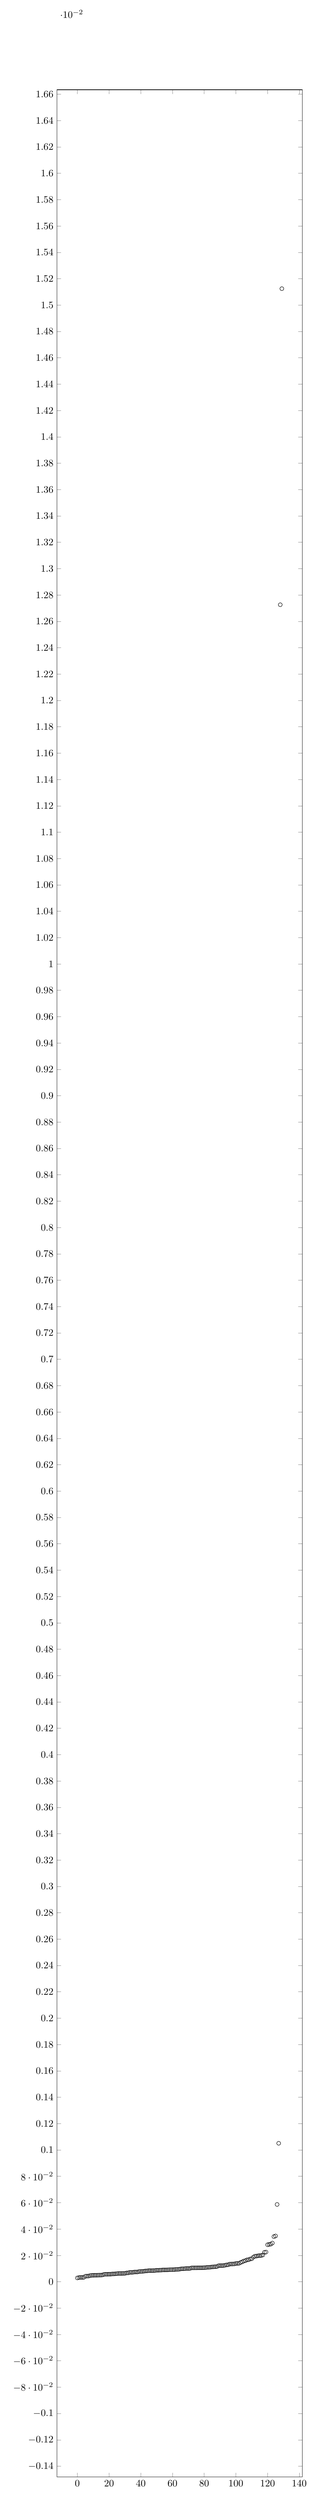
\begin{tikzpicture}
        \begin{axis}[%
        scatter/classes={%
            a={mark=o,draw=black},
            b={mark=o,draw=red}}]
        \addplot[scatter,only marks,%
            scatter src=explicit symbolic]%
        table[meta=label] {
        x y label
        0 2.8949479214654294e-05 a
        1 3.179477203046875e-05 a
        2 3.267322064601172e-05 a
        3 3.280798350852557e-05 a
        4 3.280798350852557e-05 a
        5 4.203733493201637e-05 a
        6 4.2699125166050646e-05 a
        7 4.294905342573423e-05 a
        8 4.676111584622105e-05 a
        9 4.843067177105661e-05 a
        10 4.8774191374681006e-05 a
        11 4.9445616498532656e-05 a
        12 4.9445616498532656e-05 a
        13 4.9958989436862796e-05 a
        14 5.0408826155301995e-05 a
        15 5.0408826155301995e-05 a
        16 5.193014842759746e-05 a
        17 5.634406741910958e-05 a
        18 5.6633789754044637e-05 a
        19 5.6633789754044637e-05 a
        20 5.7410217372431694e-05 a
        21 5.7410217372431694e-05 a
        22 5.921367982846027e-05 a
        23 5.921367982846027e-05 a
        24 6.0456090984576906e-05 a
        25 6.145988034834584e-05 a
        26 6.272460722809678e-05 a
        27 6.284972805645797e-05 a
        28 6.300710443137074e-05 a
        29 6.355470081318446e-05 a
        30 6.359467248323007e-05 a
        31 6.694121683315767e-05 a
        32 6.718318238640716e-05 a
        33 7.127585237345829e-05 a
        34 7.127585237345829e-05 a
        35 7.155322529164951e-05 a
        36 7.38556711976285e-05 a
        37 7.41805540625215e-05 a
        38 7.41805540625215e-05 a
        39 7.765820244366868e-05 a
        40 7.784120665026037e-05 a
        41 7.850775711089268e-05 a
        42 7.993973309373286e-05 a
        43 8.191994222015357e-05 a
        44 8.230819546665794e-05 a
        45 8.420232050680483e-05 a
        46 8.426994000106784e-05 a
        47 8.427717433224613e-05 a
        48 8.479177316626968e-05 a
        49 8.527074308148876e-05 a
        50 8.721724394873936e-05 a
        51 8.722066451929488e-05 a
        52 8.804553811338067e-05 a
        53 8.830233135155855e-05 a
        54 8.975832698738875e-05 a
        55 8.975832698738875e-05 a
        56 8.994826250782899e-05 a
        57 9.030466847320144e-05 a
        58 9.129116493983801e-05 a
        59 9.134194523707361e-05 a
        60 9.161579912448281e-05 a
        61 9.193227245685756e-05 a
        62 9.370516727749144e-05 a
        63 9.370516727749144e-05 a
        64 9.447030026752446e-05 a
        65 9.695684147183935e-05 a
        66 9.84919485426008e-05 a
        67 9.84919485426008e-05 a
        68 9.967369188253414e-05 a
        69 0.00010069773319988507 a
        70 0.00010069773319988507 a
        71 0.00010084232469055083 a
        72 0.00010512257877014406 a
        73 0.00010531121163963648 a
        74 0.00010531121163963648 a
        75 0.00010546120599483379 a
        76 0.00010572136596011746 a
        77 0.00010583143723479704 a
        78 0.00010588947949861364 a
        79 0.00010619424500734341 a
        80 0.00010702116161766447 a
        81 0.00010720818806042881 a
        82 0.00010954500810094572 a
        83 0.00010954500810094572 a
        84 0.00011073430522929063 a
        85 0.00011246416770882411 a
        86 0.0001130661635295037 a
        87 0.00011438558850046904 a
        88 0.00011469125335755415 a
        89 0.00012147392693952117 a
        90 0.00012237591171992 a
        91 0.0001224201334093466 a
        92 0.00012276203358687853 a
        93 0.0001248071419298498 a
        94 0.00012783937274188738 a
        95 0.00012853116577443856 a
        96 0.00013370751331335452 a
        97 0.00013450189840040735 a
        98 0.00013450189840040735 a
        99 0.00013535715902440975 a
        100 0.00013868052735234137 a
        101 0.00013946592819106236 a
        102 0.00013970777345427544 a
        103 0.000146505571066363 a
        104 0.00015101069658064682 a
        105 0.00015706270827900125 a
        106 0.00016013706955956582 a
        107 0.0001662494310569234 a
        108 0.0001669486955830121 a
        109 0.00017282103511564564 a
        110 0.0001741512152900111 a
        111 0.0001867419363296455 a
        112 0.00019374828758415263 a
        113 0.00019483919084249817 a
        114 0.00019699221542950795 a
        115 0.00019850109877225447 a
        116 0.00019912614342020588 a
        117 0.0002031933960156964 a
        118 0.0002232952178907816 a
        119 0.00022506654839991077 a
        120 0.000280816704139863 a
        121 0.0002832259109375601 a
        122 0.00028521681835927984 a
        123 0.00029354421334281766 a
        124 0.0003426297800563272 a
        125 0.00034744633170887413 a
        126 0.0005864789735718681 a
        127 0.0010507104872560743 a
        128 0.012726185306264882 a
        129 0.015124607637026024 a
            };
        \end{axis}
    \end{tikzpicture}
\caption{4-dist sorted graph for } \label{fig:4_dist_sorted_graph}
\end{figure}


                        \begin{figure}
                            \centering
                            \begin{tikzpicture}[]
                                \pgfplotsset{%
                                    width=.7\textwidth,
                                    height=.4\textheight
                                }
                                \begin{axis}[xlabel={Average dynamic energy consumption (Watts)}, title={Dram - Fasta - Dynamic Energy - with outliers}, ytick={1, 2, 3, 4, 5, 6, 7, 8, 9, 10, 11, 12, 13},
                                yticklabels={
                                    SP4 - IPG , SP4 - LHM , SP4 - E3 , SP4 - RAPL , SB - IPG , SB - LHM , SB - E3 , SB - RAPL , WRK - IPG , WRK - LHM , WRK - CLAMP (win) , WRK - RAPL , WRK - CLAMP (lin) 
                                    },
                                    xmin=0,xmax=80,
                                    ]
                                
                                \addplot+ [boxplot prepared={
                                lower whisker=0.10375567387783291,
                                lower quartile=0.11534461113898242,
                                median=0.11826862867259347,
                                upper quartile=0.12268613112552085,
                                upper whisker=0.14669585999344925},
                                ] table[row sep=\\,y index=0] {\\};
                                
                                \addplot+ [boxplot prepared={
                                lower whisker=0.0862842112288128,
                                lower quartile=0.10202879124519204,
                                median=0.10554987794325832,
                                upper quartile=0.10968250635173943,
                                upper whisker=0.1592616793573518},
                                ] table[row sep=\\,y index=0] {\\};
                                
                                \addplot+ [boxplot prepared={
                                lower whisker=0.0,
                                lower quartile=0.0,
                                median=0.0,
                                upper quartile=0.0,
                                upper whisker=0.0},
                                ] table[row sep=\\,y index=0] {\\};
                                
                                \addplot+ [boxplot prepared={
                                lower whisker=-58.376667674084956,
                                lower quartile=24.65499145717873,
                                median=113.55193693398685,
                                upper quartile=201.09246580893398,
                                upper whisker=285.6373247163493},
                                ] table[row sep=\\,y index=0] {\\};
                                
                                \addplot+ [boxplot prepared={
                                lower whisker=0.07774857916188005,
                                lower quartile=0.0873242550944483,
                                median=0.09508604503433815,
                                upper quartile=0.10206423245741358,
                                upper whisker=0.13756539955796498},
                                ] table[row sep=\\,y index=0] {\\};
                                
                                \addplot+ [boxplot prepared={
                                lower whisker=0.07256163691225603,
                                lower quartile=0.08089023223934655,
                                median=0.08963415201613556,
                                upper quartile=0.09406224213444994,
                                upper whisker=0.13676124570877235},
                                ] table[row sep=\\,y index=0] {\\};
                                
                                \addplot+ [boxplot prepared={
                                lower whisker=0.0,
                                lower quartile=0.0,
                                median=0.0,
                                upper quartile=0.0,
                                upper whisker=0.0},
                                ] table[row sep=\\,y index=0] {\\};
                                
                                \addplot+ [boxplot prepared={
                                lower whisker=-37.044547337624394,
                                lower quartile=-1.4124469487498352,
                                median=35.64065726225357,
                                upper quartile=72.48940753615494,
                                upper whisker=113.22179616624354},
                                ] table[row sep=\\,y index=0] {\\};
                                
                                \addplot+ [boxplot prepared={
                                lower whisker=0.013368045961463015,
                                lower quartile=0.016088896176256334,
                                median=0.01687580237366476,
                                upper quartile=0.017975615001784323,
                                upper whisker=0.10726491114142167},
                                ] table[row sep=\\,y index=0] {\\};
                                
                                \addplot+ [boxplot prepared={
                                lower whisker=0.013483540437493668,
                                lower quartile=0.016545480037850613,
                                median=0.016984038349566133,
                                upper quartile=0.01806521189896282,
                                upper whisker=0.10485184969555783},
                                ] table[row sep=\\,y index=0] {\\};
                                
                                \addplot+ [boxplot prepared={
                                lower whisker=0.0,
                                lower quartile=0.0,
                                median=0.0,
                                upper quartile=0.0,
                                upper whisker=0.0},
                                ] table[row sep=\\,y index=0] {\\};
                                
                                \addplot+ [boxplot prepared={
                                lower whisker=-4.312948877137323,
                                lower quartile=563.2009907152465,
                                median=1130.2995209910928,
                                upper quartile=1699.72830809869,
                                upper whisker=2265.3777432909205},
                                ] table[row sep=\\,y index=0] {\\};
                                
                                \addplot+ [boxplot prepared={
                                lower whisker=0.0,
                                lower quartile=0.0,
                                median=0.0,
                                upper quartile=0.0,
                                upper whisker=0.0},
                                ] table[row sep=\\,y index=0] {\\};
                                
                                \end{axis}
                            \end{tikzpicture}
                        \caption{A comparison of of Dram dynamic energy consumption for test case Fasta for all DUT's and OS's  (with outliers)} \label{fig:Fasta_Dram_comparison_dynamic_energy_with_outliers_avg_watts}
                        \end{figure}
                        

                        \begin{figure}
                            \centering
                            \begin{tikzpicture}[]
                                \pgfplotsset{%
                                    width=.7\textwidth,
                                    height=.4\textheight
                                }
                                \begin{axis}[xlabel={Average dynamic energy consumption (Watts)}, title={Dram - Fasta - Dynamic Energy - with outliers}, ytick={1, 2, 3, 4, 5, 6, 7, 8, 9, 10, 11, 12, 13},
                                yticklabels={
                                    SP4 - IPG , SP4 - LHM , SP4 - E3 , SP4 - RAPL , SB - IPG , SB - LHM , SB - E3 , SB - RAPL , WRK - IPG , WRK - LHM , WRK - CLAMP (win) , WRK - RAPL , WRK - CLAMP (lin) 
                                    },
                                    xmin=0,xmax=80,
                                    ]
                                
                                \addplot+ [boxplot prepared={
                                lower whisker=0.10375567387783291,
                                lower quartile=0.11534461113898242,
                                median=0.11826862867259347,
                                upper quartile=0.12268613112552085,
                                upper whisker=0.14669585999344925},
                                ] table[row sep=\\,y index=0] {\\};
                                
                                \addplot+ [boxplot prepared={
                                lower whisker=0.0862842112288128,
                                lower quartile=0.10202879124519204,
                                median=0.10554987794325832,
                                upper quartile=0.10968250635173943,
                                upper whisker=0.1592616793573518},
                                ] table[row sep=\\,y index=0] {\\};
                                
                                \addplot+ [boxplot prepared={
                                lower whisker=0.0,
                                lower quartile=0.0,
                                median=0.0,
                                upper quartile=0.0,
                                upper whisker=0.0},
                                ] table[row sep=\\,y index=0] {\\};
                                
                                \addplot+ [boxplot prepared={
                                lower whisker=-58.376667674084956,
                                lower quartile=24.65499145717873,
                                median=113.55193693398685,
                                upper quartile=201.09246580893398,
                                upper whisker=285.6373247163493},
                                ] table[row sep=\\,y index=0] {\\};
                                
                                \addplot+ [boxplot prepared={
                                lower whisker=0.07774857916188005,
                                lower quartile=0.0873242550944483,
                                median=0.09508604503433815,
                                upper quartile=0.10206423245741358,
                                upper whisker=0.13756539955796498},
                                ] table[row sep=\\,y index=0] {\\};
                                
                                \addplot+ [boxplot prepared={
                                lower whisker=0.07256163691225603,
                                lower quartile=0.08089023223934655,
                                median=0.08963415201613556,
                                upper quartile=0.09406224213444994,
                                upper whisker=0.13676124570877235},
                                ] table[row sep=\\,y index=0] {\\};
                                
                                \addplot+ [boxplot prepared={
                                lower whisker=0.0,
                                lower quartile=0.0,
                                median=0.0,
                                upper quartile=0.0,
                                upper whisker=0.0},
                                ] table[row sep=\\,y index=0] {\\};
                                
                                \addplot+ [boxplot prepared={
                                lower whisker=-37.044547337624394,
                                lower quartile=-1.4124469487498352,
                                median=35.64065726225357,
                                upper quartile=72.48940753615494,
                                upper whisker=113.22179616624354},
                                ] table[row sep=\\,y index=0] {\\};
                                
                                \addplot+ [boxplot prepared={
                                lower whisker=0.013368045961463015,
                                lower quartile=0.016088896176256334,
                                median=0.01687580237366476,
                                upper quartile=0.017975615001784323,
                                upper whisker=0.10726491114142167},
                                ] table[row sep=\\,y index=0] {\\};
                                
                                \addplot+ [boxplot prepared={
                                lower whisker=0.013483540437493668,
                                lower quartile=0.016545480037850613,
                                median=0.016984038349566133,
                                upper quartile=0.01806521189896282,
                                upper whisker=0.10485184969555783},
                                ] table[row sep=\\,y index=0] {\\};
                                
                                \addplot+ [boxplot prepared={
                                lower whisker=0.0,
                                lower quartile=0.0,
                                median=0.0,
                                upper quartile=0.0,
                                upper whisker=0.0},
                                ] table[row sep=\\,y index=0] {\\};
                                
                                \addplot+ [boxplot prepared={
                                lower whisker=-4.312948877137323,
                                lower quartile=563.2009907152465,
                                median=1130.2995209910928,
                                upper quartile=1699.72830809869,
                                upper whisker=2265.3777432909205},
                                ] table[row sep=\\,y index=0] {\\};
                                
                                \addplot+ [boxplot prepared={
                                lower whisker=0.0,
                                lower quartile=0.0,
                                median=0.0,
                                upper quartile=0.0,
                                upper whisker=0.0},
                                ] table[row sep=\\,y index=0] {\\};
                                
                                \end{axis}
                            \end{tikzpicture}
                        \caption{A comparison of of Dram dynamic energy consumption for test case Fasta for all DUT's and OS's  (with outliers)} \label{fig:Fasta_Dram_comparison_dynamic_energy_with_outliers_avg_watts}
                        \end{figure}
                        

                        \begin{figure}
                            \centering
                            \begin{tikzpicture}[]
                                \pgfplotsset{%
                                    width=.7\textwidth,
                                    height=.4\textheight
                                }
                                \begin{axis}[xlabel={Average dynamic energy consumption (Watts)}, title={Dram - Fasta - Dynamic Energy - with outliers}, ytick={1, 2, 3, 4, 5, 6, 7, 8, 9, 10, 11, 12, 13},
                                yticklabels={
                                    SP4 - IPG , SP4 - LHM , SP4 - E3 , SP4 - RAPL , SB - IPG , SB - LHM , SB - E3 , SB - RAPL , WRK - IPG , WRK - LHM , WRK - CLAMP (win) , WRK - RAPL , WRK - CLAMP (lin) 
                                    },
                                    xmin=0,xmax=80,
                                    ]
                                
                                \addplot+ [boxplot prepared={
                                lower whisker=0.10375567387783291,
                                lower quartile=0.11534461113898242,
                                median=0.11826862867259347,
                                upper quartile=0.12268613112552085,
                                upper whisker=0.14669585999344925},
                                ] table[row sep=\\,y index=0] {\\};
                                
                                \addplot+ [boxplot prepared={
                                lower whisker=0.0862842112288128,
                                lower quartile=0.10202879124519204,
                                median=0.10554987794325832,
                                upper quartile=0.10968250635173943,
                                upper whisker=0.1592616793573518},
                                ] table[row sep=\\,y index=0] {\\};
                                
                                \addplot+ [boxplot prepared={
                                lower whisker=0.0,
                                lower quartile=0.0,
                                median=0.0,
                                upper quartile=0.0,
                                upper whisker=0.0},
                                ] table[row sep=\\,y index=0] {\\};
                                
                                \addplot+ [boxplot prepared={
                                lower whisker=-58.376667674084956,
                                lower quartile=24.65499145717873,
                                median=113.55193693398685,
                                upper quartile=201.09246580893398,
                                upper whisker=285.6373247163493},
                                ] table[row sep=\\,y index=0] {\\};
                                
                                \addplot+ [boxplot prepared={
                                lower whisker=0.07774857916188005,
                                lower quartile=0.0873242550944483,
                                median=0.09508604503433815,
                                upper quartile=0.10206423245741358,
                                upper whisker=0.13756539955796498},
                                ] table[row sep=\\,y index=0] {\\};
                                
                                \addplot+ [boxplot prepared={
                                lower whisker=0.07256163691225603,
                                lower quartile=0.08089023223934655,
                                median=0.08963415201613556,
                                upper quartile=0.09406224213444994,
                                upper whisker=0.13676124570877235},
                                ] table[row sep=\\,y index=0] {\\};
                                
                                \addplot+ [boxplot prepared={
                                lower whisker=0.0,
                                lower quartile=0.0,
                                median=0.0,
                                upper quartile=0.0,
                                upper whisker=0.0},
                                ] table[row sep=\\,y index=0] {\\};
                                
                                \addplot+ [boxplot prepared={
                                lower whisker=-37.044547337624394,
                                lower quartile=-1.4124469487498352,
                                median=35.64065726225357,
                                upper quartile=72.48940753615494,
                                upper whisker=113.22179616624354},
                                ] table[row sep=\\,y index=0] {\\};
                                
                                \addplot+ [boxplot prepared={
                                lower whisker=0.013368045961463015,
                                lower quartile=0.016088896176256334,
                                median=0.01687580237366476,
                                upper quartile=0.017975615001784323,
                                upper whisker=0.10726491114142167},
                                ] table[row sep=\\,y index=0] {\\};
                                
                                \addplot+ [boxplot prepared={
                                lower whisker=0.013483540437493668,
                                lower quartile=0.016545480037850613,
                                median=0.016984038349566133,
                                upper quartile=0.01806521189896282,
                                upper whisker=0.10485184969555783},
                                ] table[row sep=\\,y index=0] {\\};
                                
                                \addplot+ [boxplot prepared={
                                lower whisker=0.0,
                                lower quartile=0.0,
                                median=0.0,
                                upper quartile=0.0,
                                upper whisker=0.0},
                                ] table[row sep=\\,y index=0] {\\};
                                
                                \addplot+ [boxplot prepared={
                                lower whisker=-4.312948877137323,
                                lower quartile=563.2009907152465,
                                median=1130.2995209910928,
                                upper quartile=1699.72830809869,
                                upper whisker=2265.3777432909205},
                                ] table[row sep=\\,y index=0] {\\};
                                
                                \addplot+ [boxplot prepared={
                                lower whisker=0.0,
                                lower quartile=0.0,
                                median=0.0,
                                upper quartile=0.0,
                                upper whisker=0.0},
                                ] table[row sep=\\,y index=0] {\\};
                                
                                \end{axis}
                            \end{tikzpicture}
                        \caption{A comparison of of Dram dynamic energy consumption for test case Fasta for all DUT's and OS's  (with outliers)} \label{fig:Fasta_Dram_comparison_dynamic_energy_with_outliers_avg_watts}
                        \end{figure}
                        

                        \begin{figure}
                            \centering
                            \begin{tikzpicture}[]
                                \pgfplotsset{%
                                    width=.7\textwidth,
                                    height=.4\textheight
                                }
                                \begin{axis}[xlabel={Average dynamic energy consumption (Watts)}, title={Dram - Fasta - Dynamic Energy - with outliers}, ytick={1, 2, 3, 4, 5, 6, 7, 8, 9, 10, 11, 12, 13},
                                yticklabels={
                                    SP4 - IPG , SP4 - LHM , SP4 - E3 , SP4 - RAPL , SB - IPG , SB - LHM , SB - E3 , SB - RAPL , WRK - IPG , WRK - LHM , WRK - CLAMP (win) , WRK - RAPL , WRK - CLAMP (lin) 
                                    },
                                    xmin=0,xmax=80,
                                    ]
                                
                                \addplot+ [boxplot prepared={
                                lower whisker=0.10375567387783291,
                                lower quartile=0.11534461113898242,
                                median=0.11826862867259347,
                                upper quartile=0.12268613112552085,
                                upper whisker=0.14669585999344925},
                                ] table[row sep=\\,y index=0] {\\};
                                
                                \addplot+ [boxplot prepared={
                                lower whisker=0.0862842112288128,
                                lower quartile=0.10202879124519204,
                                median=0.10554987794325832,
                                upper quartile=0.10968250635173943,
                                upper whisker=0.1592616793573518},
                                ] table[row sep=\\,y index=0] {\\};
                                
                                \addplot+ [boxplot prepared={
                                lower whisker=0.0,
                                lower quartile=0.0,
                                median=0.0,
                                upper quartile=0.0,
                                upper whisker=0.0},
                                ] table[row sep=\\,y index=0] {\\};
                                
                                \addplot+ [boxplot prepared={
                                lower whisker=-58.376667674084956,
                                lower quartile=24.65499145717873,
                                median=113.55193693398685,
                                upper quartile=201.09246580893398,
                                upper whisker=285.6373247163493},
                                ] table[row sep=\\,y index=0] {\\};
                                
                                \addplot+ [boxplot prepared={
                                lower whisker=0.07774857916188005,
                                lower quartile=0.0873242550944483,
                                median=0.09508604503433815,
                                upper quartile=0.10206423245741358,
                                upper whisker=0.13756539955796498},
                                ] table[row sep=\\,y index=0] {\\};
                                
                                \addplot+ [boxplot prepared={
                                lower whisker=0.07256163691225603,
                                lower quartile=0.08089023223934655,
                                median=0.08963415201613556,
                                upper quartile=0.09406224213444994,
                                upper whisker=0.13676124570877235},
                                ] table[row sep=\\,y index=0] {\\};
                                
                                \addplot+ [boxplot prepared={
                                lower whisker=0.0,
                                lower quartile=0.0,
                                median=0.0,
                                upper quartile=0.0,
                                upper whisker=0.0},
                                ] table[row sep=\\,y index=0] {\\};
                                
                                \addplot+ [boxplot prepared={
                                lower whisker=-37.044547337624394,
                                lower quartile=-1.4124469487498352,
                                median=35.64065726225357,
                                upper quartile=72.48940753615494,
                                upper whisker=113.22179616624354},
                                ] table[row sep=\\,y index=0] {\\};
                                
                                \addplot+ [boxplot prepared={
                                lower whisker=0.013368045961463015,
                                lower quartile=0.016088896176256334,
                                median=0.01687580237366476,
                                upper quartile=0.017975615001784323,
                                upper whisker=0.10726491114142167},
                                ] table[row sep=\\,y index=0] {\\};
                                
                                \addplot+ [boxplot prepared={
                                lower whisker=0.013483540437493668,
                                lower quartile=0.016545480037850613,
                                median=0.016984038349566133,
                                upper quartile=0.01806521189896282,
                                upper whisker=0.10485184969555783},
                                ] table[row sep=\\,y index=0] {\\};
                                
                                \addplot+ [boxplot prepared={
                                lower whisker=0.0,
                                lower quartile=0.0,
                                median=0.0,
                                upper quartile=0.0,
                                upper whisker=0.0},
                                ] table[row sep=\\,y index=0] {\\};
                                
                                \addplot+ [boxplot prepared={
                                lower whisker=-4.312948877137323,
                                lower quartile=563.2009907152465,
                                median=1130.2995209910928,
                                upper quartile=1699.72830809869,
                                upper whisker=2265.3777432909205},
                                ] table[row sep=\\,y index=0] {\\};
                                
                                \addplot+ [boxplot prepared={
                                lower whisker=0.0,
                                lower quartile=0.0,
                                median=0.0,
                                upper quartile=0.0,
                                upper whisker=0.0},
                                ] table[row sep=\\,y index=0] {\\};
                                
                                \end{axis}
                            \end{tikzpicture}
                        \caption{A comparison of of Dram dynamic energy consumption for test case Fasta for all DUT's and OS's  (with outliers)} \label{fig:Fasta_Dram_comparison_dynamic_energy_with_outliers_avg_watts}
                        \end{figure}
                        

                        \begin{figure}
                            \centering
                            \begin{tikzpicture}[]
                                \pgfplotsset{%
                                    width=.7\textwidth,
                                    height=.4\textheight
                                }
                                \begin{axis}[xlabel={Average dynamic energy consumption (Watts)}, title={Dram - Fasta - Dynamic Energy - with outliers}, ytick={1, 2, 3, 4, 5, 6, 7, 8, 9, 10, 11, 12, 13},
                                yticklabels={
                                    SP4 - IPG , SP4 - LHM , SP4 - E3 , SP4 - RAPL , SB - IPG , SB - LHM , SB - E3 , SB - RAPL , WRK - IPG , WRK - LHM , WRK - CLAMP (win) , WRK - RAPL , WRK - CLAMP (lin) 
                                    },
                                    xmin=0,xmax=80,
                                    ]
                                
                                \addplot+ [boxplot prepared={
                                lower whisker=0.10375567387783291,
                                lower quartile=0.11534461113898242,
                                median=0.11826862867259347,
                                upper quartile=0.12268613112552085,
                                upper whisker=0.14669585999344925},
                                ] table[row sep=\\,y index=0] {\\};
                                
                                \addplot+ [boxplot prepared={
                                lower whisker=0.0862842112288128,
                                lower quartile=0.10202879124519204,
                                median=0.10554987794325832,
                                upper quartile=0.10968250635173943,
                                upper whisker=0.1592616793573518},
                                ] table[row sep=\\,y index=0] {\\};
                                
                                \addplot+ [boxplot prepared={
                                lower whisker=0.0,
                                lower quartile=0.0,
                                median=0.0,
                                upper quartile=0.0,
                                upper whisker=0.0},
                                ] table[row sep=\\,y index=0] {\\};
                                
                                \addplot+ [boxplot prepared={
                                lower whisker=-58.376667674084956,
                                lower quartile=24.65499145717873,
                                median=113.55193693398685,
                                upper quartile=201.09246580893398,
                                upper whisker=285.6373247163493},
                                ] table[row sep=\\,y index=0] {\\};
                                
                                \addplot+ [boxplot prepared={
                                lower whisker=0.07774857916188005,
                                lower quartile=0.0873242550944483,
                                median=0.09508604503433815,
                                upper quartile=0.10206423245741358,
                                upper whisker=0.13756539955796498},
                                ] table[row sep=\\,y index=0] {\\};
                                
                                \addplot+ [boxplot prepared={
                                lower whisker=0.07256163691225603,
                                lower quartile=0.08089023223934655,
                                median=0.08963415201613556,
                                upper quartile=0.09406224213444994,
                                upper whisker=0.13676124570877235},
                                ] table[row sep=\\,y index=0] {\\};
                                
                                \addplot+ [boxplot prepared={
                                lower whisker=0.0,
                                lower quartile=0.0,
                                median=0.0,
                                upper quartile=0.0,
                                upper whisker=0.0},
                                ] table[row sep=\\,y index=0] {\\};
                                
                                \addplot+ [boxplot prepared={
                                lower whisker=-37.044547337624394,
                                lower quartile=-1.4124469487498352,
                                median=35.64065726225357,
                                upper quartile=72.48940753615494,
                                upper whisker=113.22179616624354},
                                ] table[row sep=\\,y index=0] {\\};
                                
                                \addplot+ [boxplot prepared={
                                lower whisker=0.013368045961463015,
                                lower quartile=0.016088896176256334,
                                median=0.01687580237366476,
                                upper quartile=0.017975615001784323,
                                upper whisker=0.10726491114142167},
                                ] table[row sep=\\,y index=0] {\\};
                                
                                \addplot+ [boxplot prepared={
                                lower whisker=0.013483540437493668,
                                lower quartile=0.016545480037850613,
                                median=0.016984038349566133,
                                upper quartile=0.01806521189896282,
                                upper whisker=0.10485184969555783},
                                ] table[row sep=\\,y index=0] {\\};
                                
                                \addplot+ [boxplot prepared={
                                lower whisker=0.0,
                                lower quartile=0.0,
                                median=0.0,
                                upper quartile=0.0,
                                upper whisker=0.0},
                                ] table[row sep=\\,y index=0] {\\};
                                
                                \addplot+ [boxplot prepared={
                                lower whisker=-4.312948877137323,
                                lower quartile=563.2009907152465,
                                median=1130.2995209910928,
                                upper quartile=1699.72830809869,
                                upper whisker=2265.3777432909205},
                                ] table[row sep=\\,y index=0] {\\};
                                
                                \addplot+ [boxplot prepared={
                                lower whisker=0.0,
                                lower quartile=0.0,
                                median=0.0,
                                upper quartile=0.0,
                                upper whisker=0.0},
                                ] table[row sep=\\,y index=0] {\\};
                                
                                \end{axis}
                            \end{tikzpicture}
                        \caption{A comparison of of Dram dynamic energy consumption for test case Fasta for all DUT's and OS's  (with outliers)} \label{fig:Fasta_Dram_comparison_dynamic_energy_with_outliers_avg_watts}
                        \end{figure}
                        


                        \begin{figure}
                            \centering
                            \begin{tikzpicture}[]
                                \pgfplotsset{%
                                    width=.85\textwidth,
                                    height=.4\textheight
                                }
                                \begin{axis}[xlabel={Average dynamic energy consumption (Watts)}, title={Cores - BinaryTrees - Dynamic Energy - with outliers}, ytick={1, 2, 3, 4, 5, 6, 7, 8, 9, 10, 11, 12, 13},
                                yticklabels={
                                    SP4 - IPG , SP4 - LHM , SP4 - E3 , SP4 - RAPL , SB - IPG , SB - LHM , SB - E3 , SB - RAPL , WRK - IPG , WRK - LHM , WRK - CLAMP (win) , WRK - RAPL , WRK - CLAMP (lin) 
                                    },
                                    xmin=0,xmax=80,
                                    ]
                                
                                \addplot+ [boxplot prepared={
                                lower whisker=11.420748362866629,
                                lower quartile=12.6580266708996,
                                median=13.130573674940711,
                                upper quartile=13.607831789003136,
                                upper whisker=14.46411097772971},
                                ] table[row sep=\\,y index=0] {\\};
                                
                                \addplot+ [boxplot prepared={
                                lower whisker=11.376920355725565,
                                lower quartile=11.859438510771918,
                                median=12.021494244664462,
                                upper quartile=12.198808082967586,
                                upper whisker=12.733883887273084},
                                ] table[row sep=\\,y index=0] {\\};
                                
                                \addplot+ [boxplot prepared={
                                lower whisker=11.219893282713638,
                                lower quartile=11.392272070684548,
                                median=11.517371341746154,
                                upper quartile=11.621194830198572,
                                upper whisker=11.904963494099112},
                                ] table[row sep=\\,y index=0] {\\};
                                
                                \addplot+ [boxplot prepared={
                                lower whisker=7.858040649665969,
                                lower quartile=8.009985603972664,
                                median=8.035629334355505,
                                upper quartile=8.056069699901885,
                                upper whisker=8.115869058828618},
                                ] table[row sep=\\,y index=0] {\\};
                                
                                \addplot+ [boxplot prepared={
                                lower whisker=2.262212420881607,
                                lower quartile=2.665594787259187,
                                median=3.0824671350351713,
                                upper quartile=4.358960214695252,
                                upper whisker=6.1735648226258775},
                                ] table[row sep=\\,y index=0] {\\};
                                
                                \addplot+ [boxplot prepared={
                                lower whisker=1.3655759382792674,
                                lower quartile=2.523121921079479,
                                median=3.3460963285486782,
                                upper quartile=4.425424940316596,
                                upper whisker=6.272376418833985},
                                ] table[row sep=\\,y index=0] {\\};
                                
                                \addplot+ [boxplot prepared={
                                lower whisker=2.3566196168660305,
                                lower quartile=3.3153296051298047,
                                median=4.085362353031364,
                                upper quartile=4.835337745266552,
                                upper whisker=6.151594431657646},
                                ] table[row sep=\\,y index=0] {\\};
                                
                                \addplot+ [boxplot prepared={
                                lower whisker=4.828483342208097,
                                lower quartile=4.964034824723491,
                                median=5.116431256812656,
                                upper quartile=5.289743479362281,
                                upper whisker=5.625244550954983},
                                ] table[row sep=\\,y index=0] {\\};
                                
                                \addplot+ [boxplot prepared={
                                lower whisker=66.89792094118035,
                                lower quartile=67.82648820588565,
                                median=68.22365397596283,
                                upper quartile=68.53649902422302,
                                upper whisker=72.91899239828562},
                                ] table[row sep=\\,y index=0] {\\};
                                
                                \addplot+ [boxplot prepared={
                                lower whisker=65.4708069509544,
                                lower quartile=66.11534816821023,
                                median=66.27532723833454,
                                upper quartile=66.44412633159524,
                                upper whisker=69.64149630164013},
                                ] table[row sep=\\,y index=0] {\\};
                                
                                \addplot+ [boxplot prepared={
                                lower whisker=49.36748648899456,
                                lower quartile=59.39957521748035,
                                median=60.22154751822312,
                                upper quartile=68.57561563020016,
                                upper whisker=76.59487529684452},
                                ] table[row sep=\\,y index=0] {\\};
                                
                                \addplot+ [boxplot prepared={
                                lower whisker=56.400276110515385,
                                lower quartile=56.75939325693689,
                                median=56.86448126331913,
                                upper quartile=56.965123398456655,
                                upper whisker=57.15490760460869},
                                ] table[row sep=\\,y index=0] {\\};
                                
                                \addplot+ [boxplot prepared={
                                lower whisker=34.2500767117359,
                                lower quartile=51.50619275990899,
                                median=52.32916789904128,
                                upper quartile=52.74930164067668,
                                upper whisker=72.15287309502655},
                                ] table[row sep=\\,y index=0] {\\};
                                
                                \end{axis}
                            \end{tikzpicture}
                        \caption{A comparison of Cores dynamic energy consumption for test case BinaryTrees for all DUT's and OS's  (with outliers)} \label{fig:BinaryTrees_Cores_comparison_dynamic_energy_with_outliers_avg_watts}
                        \end{figure}
                        

                        \begin{figure}
                            \centering
                            \begin{tikzpicture}[]
                                \pgfplotsset{%
                                    width=.7\textwidth,
                                    height=.4\textheight
                                }
                                \begin{axis}[xlabel={Average dynamic energy consumption (Watts)}, title={Dram - Fasta - Dynamic Energy - with outliers}, ytick={1, 2, 3, 4, 5, 6, 7, 8, 9, 10, 11, 12, 13},
                                yticklabels={
                                    SP4 - IPG , SP4 - LHM , SP4 - E3 , SP4 - RAPL , SB - IPG , SB - LHM , SB - E3 , SB - RAPL , WRK - IPG , WRK - LHM , WRK - CLAMP (win) , WRK - RAPL , WRK - CLAMP (lin) 
                                    },
                                    xmin=0,xmax=80,
                                    ]
                                
                                \addplot+ [boxplot prepared={
                                lower whisker=0.10375567387783291,
                                lower quartile=0.11534461113898242,
                                median=0.11826862867259347,
                                upper quartile=0.12268613112552085,
                                upper whisker=0.14669585999344925},
                                ] table[row sep=\\,y index=0] {\\};
                                
                                \addplot+ [boxplot prepared={
                                lower whisker=0.0862842112288128,
                                lower quartile=0.10202879124519204,
                                median=0.10554987794325832,
                                upper quartile=0.10968250635173943,
                                upper whisker=0.1592616793573518},
                                ] table[row sep=\\,y index=0] {\\};
                                
                                \addplot+ [boxplot prepared={
                                lower whisker=0.0,
                                lower quartile=0.0,
                                median=0.0,
                                upper quartile=0.0,
                                upper whisker=0.0},
                                ] table[row sep=\\,y index=0] {\\};
                                
                                \addplot+ [boxplot prepared={
                                lower whisker=-58.376667674084956,
                                lower quartile=24.65499145717873,
                                median=113.55193693398685,
                                upper quartile=201.09246580893398,
                                upper whisker=285.6373247163493},
                                ] table[row sep=\\,y index=0] {\\};
                                
                                \addplot+ [boxplot prepared={
                                lower whisker=0.07774857916188005,
                                lower quartile=0.0873242550944483,
                                median=0.09508604503433815,
                                upper quartile=0.10206423245741358,
                                upper whisker=0.13756539955796498},
                                ] table[row sep=\\,y index=0] {\\};
                                
                                \addplot+ [boxplot prepared={
                                lower whisker=0.07256163691225603,
                                lower quartile=0.08089023223934655,
                                median=0.08963415201613556,
                                upper quartile=0.09406224213444994,
                                upper whisker=0.13676124570877235},
                                ] table[row sep=\\,y index=0] {\\};
                                
                                \addplot+ [boxplot prepared={
                                lower whisker=0.0,
                                lower quartile=0.0,
                                median=0.0,
                                upper quartile=0.0,
                                upper whisker=0.0},
                                ] table[row sep=\\,y index=0] {\\};
                                
                                \addplot+ [boxplot prepared={
                                lower whisker=-37.044547337624394,
                                lower quartile=-1.4124469487498352,
                                median=35.64065726225357,
                                upper quartile=72.48940753615494,
                                upper whisker=113.22179616624354},
                                ] table[row sep=\\,y index=0] {\\};
                                
                                \addplot+ [boxplot prepared={
                                lower whisker=0.013368045961463015,
                                lower quartile=0.016088896176256334,
                                median=0.01687580237366476,
                                upper quartile=0.017975615001784323,
                                upper whisker=0.10726491114142167},
                                ] table[row sep=\\,y index=0] {\\};
                                
                                \addplot+ [boxplot prepared={
                                lower whisker=0.013483540437493668,
                                lower quartile=0.016545480037850613,
                                median=0.016984038349566133,
                                upper quartile=0.01806521189896282,
                                upper whisker=0.10485184969555783},
                                ] table[row sep=\\,y index=0] {\\};
                                
                                \addplot+ [boxplot prepared={
                                lower whisker=0.0,
                                lower quartile=0.0,
                                median=0.0,
                                upper quartile=0.0,
                                upper whisker=0.0},
                                ] table[row sep=\\,y index=0] {\\};
                                
                                \addplot+ [boxplot prepared={
                                lower whisker=-4.312948877137323,
                                lower quartile=563.2009907152465,
                                median=1130.2995209910928,
                                upper quartile=1699.72830809869,
                                upper whisker=2265.3777432909205},
                                ] table[row sep=\\,y index=0] {\\};
                                
                                \addplot+ [boxplot prepared={
                                lower whisker=0.0,
                                lower quartile=0.0,
                                median=0.0,
                                upper quartile=0.0,
                                upper whisker=0.0},
                                ] table[row sep=\\,y index=0] {\\};
                                
                                \end{axis}
                            \end{tikzpicture}
                        \caption{A comparison of of Dram dynamic energy consumption for test case Fasta for all DUT's and OS's  (with outliers)} \label{fig:Fasta_Dram_comparison_dynamic_energy_with_outliers_avg_watts}
                        \end{figure}
                        

                            \begin{figure}
                                \centering
                                \begin{tikzpicture}[]
                                    \pgfplotsset{%
                                        width=.85\textwidth,
                                        height=.15\textheight
                                    }
                                    \begin{axis}[xlabel={Average energy consumption (Watts)}, title={Cores - Nbody - Energy - with outliers}, ytick={1, 2, 3, 4},
                                    yticklabels={
                                        IPG , LHM , E3 , RAPL 
                                        },
                                        xmin=0,xmax=10,
                                        ]
                                    
                                    \addplot+ [boxplot prepared={
                                    lower whisker=3.3904966623857957,
                                    lower quartile=3.590049859121917,
                                    median=3.659495158384077,
                                    upper quartile=3.7265303388398676,
                                    upper whisker=3.961455824832631},
                                    ] table[row sep=\\,y index=0] {\\};
                                    
                                    \addplot+ [boxplot prepared={
                                    lower whisker=4.310300897881025,
                                    lower quartile=4.399235063852297,
                                    median=4.436051030948529,
                                    upper quartile=4.4760085282539865,
                                    upper whisker=4.578699108862436},
                                    ] table[row sep=\\,y index=0] {\\};
                                    
                                    \addplot+ [boxplot prepared={
                                    lower whisker=2.399996038382789,
                                    lower quartile=4.241702359737292,
                                    median=4.27199328109721,
                                    upper quartile=4.302908157167919,
                                    upper whisker=4.369796102164826},
                                    ] table[row sep=\\,y index=0] {\\};
                                    
                                    \addplot+ [boxplot prepared={
                                    lower whisker=8.442268947178363,
                                    lower quartile=8.469458770450048,
                                    median=8.486493968102357,
                                    upper quartile=8.50282879621,
                                    upper whisker=8.548467746233305},
                                    ] table[row sep=\\,y index=0] {\\};
                                    
                                    \end{axis}
                                \end{tikzpicture}
                            \caption{A comparison of of Cores energy consumption for test case Nbody for the SurfaceBook,  (with outliers)} \label{fig:Nbody_Cores_comparison_energy_with_outliers_SurfaceBook_avg_watts}
                            \end{figure}
                            

                            \begin{figure}
                                \centering
                                \begin{tikzpicture}[]
                                    \pgfplotsset{%
                                        width=.7\textwidth,
                                        height=.15\textheight
                                    }
                                    \begin{axis}[xlabel={Average dynamic energy consumption (Watts)}, title={Dram - FannkuchRedux - Dynamic Energy - without outliers}, ytick={1, 2, 3},
                                    yticklabels={
                                        IntelPowerGadget , HardwareMonitor , RAPL 
                                        },
                                        xmin=0,xmax=10,
                                        ]
                                    
                                    \addplot+ [boxplot prepared={
                                    lower whisker=0.20538501792059694,
                                    lower quartile=0.21746331766250407,
                                    median=0.22181397206089515,
                                    upper quartile=0.22689881660268849,
                                    upper whisker=0.2574096342559279},
                                    ] table[row sep=\\,y index=0] {\\};
                                    
                                    \addplot+ [boxplot prepared={
                                    lower whisker=0.20011075295825292,
                                    lower quartile=0.21351009682521976,
                                    median=0.21882287282828888,
                                    upper quartile=0.22279414070357745,
                                    upper whisker=0.24916373243628814},
                                    ] table[row sep=\\,y index=0] {\\};
                                    
                                    \addplot+ [boxplot prepared={
                                    lower whisker=-36.9590502759173,
                                    lower quartile=0.42743760995280056,
                                    median=36.77656912882534,
                                    upper quartile=76.49716528340782,
                                    upper whisker=116.30089979379153},
                                    ] table[row sep=\\,y index=0] {\\};
                                    
                                    \end{axis}
                                \end{tikzpicture}
                            \caption{A comparison of of Dram dynamic energy consumption for test case FannkuchRedux for the SurfaceBook (without outliers)} \label{fig:FannkuchRedux_Dram_comparison_dynamic_energy_without_outliers_SurfaceBook_avg_watts}
                            \end{figure}
                            


                            \begin{figure}
                                \centering
                                \begin{tikzpicture}[]
                                    \pgfplotsset{%
                                        width=.7\textwidth,
                                        height=.15\textheight
                                    }
                                    \begin{axis}[xlabel={Average dynamic energy consumption (Watts)}, title={Dram - FannkuchRedux - Dynamic Energy - without outliers}, ytick={1, 2, 3},
                                    yticklabels={
                                        IntelPowerGadget , HardwareMonitor , RAPL 
                                        },
                                        xmin=0,xmax=10,
                                        ]
                                    
                                    \addplot+ [boxplot prepared={
                                    lower whisker=0.20538501792059694,
                                    lower quartile=0.21746331766250407,
                                    median=0.22181397206089515,
                                    upper quartile=0.22689881660268849,
                                    upper whisker=0.2574096342559279},
                                    ] table[row sep=\\,y index=0] {\\};
                                    
                                    \addplot+ [boxplot prepared={
                                    lower whisker=0.20011075295825292,
                                    lower quartile=0.21351009682521976,
                                    median=0.21882287282828888,
                                    upper quartile=0.22279414070357745,
                                    upper whisker=0.24916373243628814},
                                    ] table[row sep=\\,y index=0] {\\};
                                    
                                    \addplot+ [boxplot prepared={
                                    lower whisker=-36.9590502759173,
                                    lower quartile=0.42743760995280056,
                                    median=36.77656912882534,
                                    upper quartile=76.49716528340782,
                                    upper whisker=116.30089979379153},
                                    ] table[row sep=\\,y index=0] {\\};
                                    
                                    \end{axis}
                                \end{tikzpicture}
                            \caption{A comparison of of Dram dynamic energy consumption for test case FannkuchRedux for the SurfaceBook (without outliers)} \label{fig:FannkuchRedux_Dram_comparison_dynamic_energy_without_outliers_SurfaceBook_avg_watts}
                            \end{figure}
                            

                        \begin{figure}
                            \centering
                            \begin{tikzpicture}[]
                                \pgfplotsset{%
                                    width=.85\textwidth,
                                    height=.4\textheight
                                }
                                \begin{axis}[xlabel={Average dynamic energy consumption (Watts)}, title={Cores - BinaryTrees - Dynamic Energy - with outliers}, ytick={1, 2, 3, 4, 5, 6, 7, 8, 9, 10, 11, 12, 13},
                                yticklabels={
                                    SP4 - IPG , SP4 - LHM , SP4 - E3 , SP4 - RAPL , SB - IPG , SB - LHM , SB - E3 , SB - RAPL , WRK - IPG , WRK - LHM , WRK - CLAMP (win) , WRK - RAPL , WRK - CLAMP (lin) 
                                    },
                                    xmin=0,xmax=80,
                                    ]
                                
                                \addplot+ [boxplot prepared={
                                lower whisker=11.420748362866629,
                                lower quartile=12.6580266708996,
                                median=13.130573674940711,
                                upper quartile=13.607831789003136,
                                upper whisker=14.46411097772971},
                                ] table[row sep=\\,y index=0] {\\};
                                
                                \addplot+ [boxplot prepared={
                                lower whisker=11.376920355725565,
                                lower quartile=11.859438510771918,
                                median=12.021494244664462,
                                upper quartile=12.198808082967586,
                                upper whisker=12.733883887273084},
                                ] table[row sep=\\,y index=0] {\\};
                                
                                \addplot+ [boxplot prepared={
                                lower whisker=11.219893282713638,
                                lower quartile=11.392272070684548,
                                median=11.517371341746154,
                                upper quartile=11.621194830198572,
                                upper whisker=11.904963494099112},
                                ] table[row sep=\\,y index=0] {\\};
                                
                                \addplot+ [boxplot prepared={
                                lower whisker=7.858040649665969,
                                lower quartile=8.009985603972664,
                                median=8.035629334355505,
                                upper quartile=8.056069699901885,
                                upper whisker=8.115869058828618},
                                ] table[row sep=\\,y index=0] {\\};
                                
                                \addplot+ [boxplot prepared={
                                lower whisker=2.262212420881607,
                                lower quartile=2.665594787259187,
                                median=3.0824671350351713,
                                upper quartile=4.358960214695252,
                                upper whisker=6.1735648226258775},
                                ] table[row sep=\\,y index=0] {\\};
                                
                                \addplot+ [boxplot prepared={
                                lower whisker=1.3655759382792674,
                                lower quartile=2.523121921079479,
                                median=3.3460963285486782,
                                upper quartile=4.425424940316596,
                                upper whisker=6.272376418833985},
                                ] table[row sep=\\,y index=0] {\\};
                                
                                \addplot+ [boxplot prepared={
                                lower whisker=2.3566196168660305,
                                lower quartile=3.3153296051298047,
                                median=4.085362353031364,
                                upper quartile=4.835337745266552,
                                upper whisker=6.151594431657646},
                                ] table[row sep=\\,y index=0] {\\};
                                
                                \addplot+ [boxplot prepared={
                                lower whisker=4.828483342208097,
                                lower quartile=4.964034824723491,
                                median=5.116431256812656,
                                upper quartile=5.289743479362281,
                                upper whisker=5.625244550954983},
                                ] table[row sep=\\,y index=0] {\\};
                                
                                \addplot+ [boxplot prepared={
                                lower whisker=66.89792094118035,
                                lower quartile=67.82648820588565,
                                median=68.22365397596283,
                                upper quartile=68.53649902422302,
                                upper whisker=72.91899239828562},
                                ] table[row sep=\\,y index=0] {\\};
                                
                                \addplot+ [boxplot prepared={
                                lower whisker=65.4708069509544,
                                lower quartile=66.11534816821023,
                                median=66.27532723833454,
                                upper quartile=66.44412633159524,
                                upper whisker=69.64149630164013},
                                ] table[row sep=\\,y index=0] {\\};
                                
                                \addplot+ [boxplot prepared={
                                lower whisker=49.36748648899456,
                                lower quartile=59.39957521748035,
                                median=60.22154751822312,
                                upper quartile=68.57561563020016,
                                upper whisker=76.59487529684452},
                                ] table[row sep=\\,y index=0] {\\};
                                
                                \addplot+ [boxplot prepared={
                                lower whisker=56.400276110515385,
                                lower quartile=56.75939325693689,
                                median=56.86448126331913,
                                upper quartile=56.965123398456655,
                                upper whisker=57.15490760460869},
                                ] table[row sep=\\,y index=0] {\\};
                                
                                \addplot+ [boxplot prepared={
                                lower whisker=34.2500767117359,
                                lower quartile=51.50619275990899,
                                median=52.32916789904128,
                                upper quartile=52.74930164067668,
                                upper whisker=72.15287309502655},
                                ] table[row sep=\\,y index=0] {\\};
                                
                                \end{axis}
                            \end{tikzpicture}
                        \caption{A comparison of Cores dynamic energy consumption for test case BinaryTrees for all DUT's and OS's  (with outliers)} \label{fig:BinaryTrees_Cores_comparison_dynamic_energy_with_outliers_avg_watts}
                        \end{figure}
                        

                        \begin{figure}
                            \centering
                            \begin{tikzpicture}[]
                                \pgfplotsset{%
                                    width=.7\textwidth,
                                    height=.4\textheight
                                }
                                \begin{axis}[xlabel={Average dynamic energy consumption (Watts)}, title={Dram - Fasta - Dynamic Energy - with outliers}, ytick={1, 2, 3, 4, 5, 6, 7, 8, 9, 10, 11, 12, 13},
                                yticklabels={
                                    SP4 - IPG , SP4 - LHM , SP4 - E3 , SP4 - RAPL , SB - IPG , SB - LHM , SB - E3 , SB - RAPL , WRK - IPG , WRK - LHM , WRK - CLAMP (win) , WRK - RAPL , WRK - CLAMP (lin) 
                                    },
                                    xmin=0,xmax=80,
                                    ]
                                
                                \addplot+ [boxplot prepared={
                                lower whisker=0.10375567387783291,
                                lower quartile=0.11534461113898242,
                                median=0.11826862867259347,
                                upper quartile=0.12268613112552085,
                                upper whisker=0.14669585999344925},
                                ] table[row sep=\\,y index=0] {\\};
                                
                                \addplot+ [boxplot prepared={
                                lower whisker=0.0862842112288128,
                                lower quartile=0.10202879124519204,
                                median=0.10554987794325832,
                                upper quartile=0.10968250635173943,
                                upper whisker=0.1592616793573518},
                                ] table[row sep=\\,y index=0] {\\};
                                
                                \addplot+ [boxplot prepared={
                                lower whisker=0.0,
                                lower quartile=0.0,
                                median=0.0,
                                upper quartile=0.0,
                                upper whisker=0.0},
                                ] table[row sep=\\,y index=0] {\\};
                                
                                \addplot+ [boxplot prepared={
                                lower whisker=-58.376667674084956,
                                lower quartile=24.65499145717873,
                                median=113.55193693398685,
                                upper quartile=201.09246580893398,
                                upper whisker=285.6373247163493},
                                ] table[row sep=\\,y index=0] {\\};
                                
                                \addplot+ [boxplot prepared={
                                lower whisker=0.07774857916188005,
                                lower quartile=0.0873242550944483,
                                median=0.09508604503433815,
                                upper quartile=0.10206423245741358,
                                upper whisker=0.13756539955796498},
                                ] table[row sep=\\,y index=0] {\\};
                                
                                \addplot+ [boxplot prepared={
                                lower whisker=0.07256163691225603,
                                lower quartile=0.08089023223934655,
                                median=0.08963415201613556,
                                upper quartile=0.09406224213444994,
                                upper whisker=0.13676124570877235},
                                ] table[row sep=\\,y index=0] {\\};
                                
                                \addplot+ [boxplot prepared={
                                lower whisker=0.0,
                                lower quartile=0.0,
                                median=0.0,
                                upper quartile=0.0,
                                upper whisker=0.0},
                                ] table[row sep=\\,y index=0] {\\};
                                
                                \addplot+ [boxplot prepared={
                                lower whisker=-37.044547337624394,
                                lower quartile=-1.4124469487498352,
                                median=35.64065726225357,
                                upper quartile=72.48940753615494,
                                upper whisker=113.22179616624354},
                                ] table[row sep=\\,y index=0] {\\};
                                
                                \addplot+ [boxplot prepared={
                                lower whisker=0.013368045961463015,
                                lower quartile=0.016088896176256334,
                                median=0.01687580237366476,
                                upper quartile=0.017975615001784323,
                                upper whisker=0.10726491114142167},
                                ] table[row sep=\\,y index=0] {\\};
                                
                                \addplot+ [boxplot prepared={
                                lower whisker=0.013483540437493668,
                                lower quartile=0.016545480037850613,
                                median=0.016984038349566133,
                                upper quartile=0.01806521189896282,
                                upper whisker=0.10485184969555783},
                                ] table[row sep=\\,y index=0] {\\};
                                
                                \addplot+ [boxplot prepared={
                                lower whisker=0.0,
                                lower quartile=0.0,
                                median=0.0,
                                upper quartile=0.0,
                                upper whisker=0.0},
                                ] table[row sep=\\,y index=0] {\\};
                                
                                \addplot+ [boxplot prepared={
                                lower whisker=-4.312948877137323,
                                lower quartile=563.2009907152465,
                                median=1130.2995209910928,
                                upper quartile=1699.72830809869,
                                upper whisker=2265.3777432909205},
                                ] table[row sep=\\,y index=0] {\\};
                                
                                \addplot+ [boxplot prepared={
                                lower whisker=0.0,
                                lower quartile=0.0,
                                median=0.0,
                                upper quartile=0.0,
                                upper whisker=0.0},
                                ] table[row sep=\\,y index=0] {\\};
                                
                                \end{axis}
                            \end{tikzpicture}
                        \caption{A comparison of of Dram dynamic energy consumption for test case Fasta for all DUT's and OS's  (with outliers)} \label{fig:Fasta_Dram_comparison_dynamic_energy_with_outliers_avg_watts}
                        \end{figure}
                        

                            \begin{figure}
                                \centering
                                \begin{tikzpicture}[]
                                    \pgfplotsset{%
                                        width=.85\textwidth,
                                        height=.15\textheight
                                    }
                                    \begin{axis}[xlabel={Average energy consumption (Watts)}, title={Cores - Nbody - Energy - with outliers}, ytick={1, 2, 3, 4},
                                    yticklabels={
                                        IPG , LHM , E3 , RAPL 
                                        },
                                        xmin=0,xmax=10,
                                        ]
                                    
                                    \addplot+ [boxplot prepared={
                                    lower whisker=3.3904966623857957,
                                    lower quartile=3.590049859121917,
                                    median=3.659495158384077,
                                    upper quartile=3.7265303388398676,
                                    upper whisker=3.961455824832631},
                                    ] table[row sep=\\,y index=0] {\\};
                                    
                                    \addplot+ [boxplot prepared={
                                    lower whisker=4.310300897881025,
                                    lower quartile=4.399235063852297,
                                    median=4.436051030948529,
                                    upper quartile=4.4760085282539865,
                                    upper whisker=4.578699108862436},
                                    ] table[row sep=\\,y index=0] {\\};
                                    
                                    \addplot+ [boxplot prepared={
                                    lower whisker=2.399996038382789,
                                    lower quartile=4.241702359737292,
                                    median=4.27199328109721,
                                    upper quartile=4.302908157167919,
                                    upper whisker=4.369796102164826},
                                    ] table[row sep=\\,y index=0] {\\};
                                    
                                    \addplot+ [boxplot prepared={
                                    lower whisker=8.442268947178363,
                                    lower quartile=8.469458770450048,
                                    median=8.486493968102357,
                                    upper quartile=8.50282879621,
                                    upper whisker=8.548467746233305},
                                    ] table[row sep=\\,y index=0] {\\};
                                    
                                    \end{axis}
                                \end{tikzpicture}
                            \caption{A comparison of of Cores energy consumption for test case Nbody for the SurfaceBook,  (with outliers)} \label{fig:Nbody_Cores_comparison_energy_with_outliers_SurfaceBook_avg_watts}
                            \end{figure}
                            


                        \begin{figure}
                            \centering
                            \begin{tikzpicture}[]
                                \pgfplotsset{%
                                    width=.85\textwidth,
                                    height=.4\textheight
                                }
                                \begin{axis}[xlabel={Average dynamic energy consumption (Watts)}, title={Cores - BinaryTrees - Dynamic Energy - with outliers}, ytick={1, 2, 3, 4, 5, 6, 7, 8, 9, 10, 11, 12, 13},
                                yticklabels={
                                    SP4 - IPG , SP4 - LHM , SP4 - E3 , SP4 - RAPL , SB - IPG , SB - LHM , SB - E3 , SB - RAPL , WRK - IPG , WRK - LHM , WRK - CLAMP (win) , WRK - RAPL , WRK - CLAMP (lin) 
                                    },
                                    xmin=0,xmax=80,
                                    ]
                                
                                \addplot+ [boxplot prepared={
                                lower whisker=11.420748362866629,
                                lower quartile=12.6580266708996,
                                median=13.130573674940711,
                                upper quartile=13.607831789003136,
                                upper whisker=14.46411097772971},
                                ] table[row sep=\\,y index=0] {\\};
                                
                                \addplot+ [boxplot prepared={
                                lower whisker=11.376920355725565,
                                lower quartile=11.859438510771918,
                                median=12.021494244664462,
                                upper quartile=12.198808082967586,
                                upper whisker=12.733883887273084},
                                ] table[row sep=\\,y index=0] {\\};
                                
                                \addplot+ [boxplot prepared={
                                lower whisker=11.219893282713638,
                                lower quartile=11.392272070684548,
                                median=11.517371341746154,
                                upper quartile=11.621194830198572,
                                upper whisker=11.904963494099112},
                                ] table[row sep=\\,y index=0] {\\};
                                
                                \addplot+ [boxplot prepared={
                                lower whisker=7.858040649665969,
                                lower quartile=8.009985603972664,
                                median=8.035629334355505,
                                upper quartile=8.056069699901885,
                                upper whisker=8.115869058828618},
                                ] table[row sep=\\,y index=0] {\\};
                                
                                \addplot+ [boxplot prepared={
                                lower whisker=2.262212420881607,
                                lower quartile=2.665594787259187,
                                median=3.0824671350351713,
                                upper quartile=4.358960214695252,
                                upper whisker=6.1735648226258775},
                                ] table[row sep=\\,y index=0] {\\};
                                
                                \addplot+ [boxplot prepared={
                                lower whisker=1.3655759382792674,
                                lower quartile=2.523121921079479,
                                median=3.3460963285486782,
                                upper quartile=4.425424940316596,
                                upper whisker=6.272376418833985},
                                ] table[row sep=\\,y index=0] {\\};
                                
                                \addplot+ [boxplot prepared={
                                lower whisker=2.3566196168660305,
                                lower quartile=3.3153296051298047,
                                median=4.085362353031364,
                                upper quartile=4.835337745266552,
                                upper whisker=6.151594431657646},
                                ] table[row sep=\\,y index=0] {\\};
                                
                                \addplot+ [boxplot prepared={
                                lower whisker=4.828483342208097,
                                lower quartile=4.964034824723491,
                                median=5.116431256812656,
                                upper quartile=5.289743479362281,
                                upper whisker=5.625244550954983},
                                ] table[row sep=\\,y index=0] {\\};
                                
                                \addplot+ [boxplot prepared={
                                lower whisker=66.89792094118035,
                                lower quartile=67.82648820588565,
                                median=68.22365397596283,
                                upper quartile=68.53649902422302,
                                upper whisker=72.91899239828562},
                                ] table[row sep=\\,y index=0] {\\};
                                
                                \addplot+ [boxplot prepared={
                                lower whisker=65.4708069509544,
                                lower quartile=66.11534816821023,
                                median=66.27532723833454,
                                upper quartile=66.44412633159524,
                                upper whisker=69.64149630164013},
                                ] table[row sep=\\,y index=0] {\\};
                                
                                \addplot+ [boxplot prepared={
                                lower whisker=49.36748648899456,
                                lower quartile=59.39957521748035,
                                median=60.22154751822312,
                                upper quartile=68.57561563020016,
                                upper whisker=76.59487529684452},
                                ] table[row sep=\\,y index=0] {\\};
                                
                                \addplot+ [boxplot prepared={
                                lower whisker=56.400276110515385,
                                lower quartile=56.75939325693689,
                                median=56.86448126331913,
                                upper quartile=56.965123398456655,
                                upper whisker=57.15490760460869},
                                ] table[row sep=\\,y index=0] {\\};
                                
                                \addplot+ [boxplot prepared={
                                lower whisker=34.2500767117359,
                                lower quartile=51.50619275990899,
                                median=52.32916789904128,
                                upper quartile=52.74930164067668,
                                upper whisker=72.15287309502655},
                                ] table[row sep=\\,y index=0] {\\};
                                
                                \end{axis}
                            \end{tikzpicture}
                        \caption{A comparison of Cores dynamic energy consumption for test case BinaryTrees for all DUT's and OS's  (with outliers)} \label{fig:BinaryTrees_Cores_comparison_dynamic_energy_with_outliers_avg_watts}
                        \end{figure}
                        

                        \begin{figure}
                            \centering
                            \begin{tikzpicture}[]
                                \pgfplotsset{%
                                    width=.7\textwidth,
                                    height=.4\textheight
                                }
                                \begin{axis}[xlabel={Average dynamic energy consumption (Watts)}, title={Dram - Fasta - Dynamic Energy - with outliers}, ytick={1, 2, 3, 4, 5, 6, 7, 8, 9, 10, 11, 12, 13},
                                yticklabels={
                                    SP4 - IPG , SP4 - LHM , SP4 - E3 , SP4 - RAPL , SB - IPG , SB - LHM , SB - E3 , SB - RAPL , WRK - IPG , WRK - LHM , WRK - CLAMP (win) , WRK - RAPL , WRK - CLAMP (lin) 
                                    },
                                    xmin=0,xmax=80,
                                    ]
                                
                                \addplot+ [boxplot prepared={
                                lower whisker=0.10375567387783291,
                                lower quartile=0.11534461113898242,
                                median=0.11826862867259347,
                                upper quartile=0.12268613112552085,
                                upper whisker=0.14669585999344925},
                                ] table[row sep=\\,y index=0] {\\};
                                
                                \addplot+ [boxplot prepared={
                                lower whisker=0.0862842112288128,
                                lower quartile=0.10202879124519204,
                                median=0.10554987794325832,
                                upper quartile=0.10968250635173943,
                                upper whisker=0.1592616793573518},
                                ] table[row sep=\\,y index=0] {\\};
                                
                                \addplot+ [boxplot prepared={
                                lower whisker=0.0,
                                lower quartile=0.0,
                                median=0.0,
                                upper quartile=0.0,
                                upper whisker=0.0},
                                ] table[row sep=\\,y index=0] {\\};
                                
                                \addplot+ [boxplot prepared={
                                lower whisker=-58.376667674084956,
                                lower quartile=24.65499145717873,
                                median=113.55193693398685,
                                upper quartile=201.09246580893398,
                                upper whisker=285.6373247163493},
                                ] table[row sep=\\,y index=0] {\\};
                                
                                \addplot+ [boxplot prepared={
                                lower whisker=0.07774857916188005,
                                lower quartile=0.0873242550944483,
                                median=0.09508604503433815,
                                upper quartile=0.10206423245741358,
                                upper whisker=0.13756539955796498},
                                ] table[row sep=\\,y index=0] {\\};
                                
                                \addplot+ [boxplot prepared={
                                lower whisker=0.07256163691225603,
                                lower quartile=0.08089023223934655,
                                median=0.08963415201613556,
                                upper quartile=0.09406224213444994,
                                upper whisker=0.13676124570877235},
                                ] table[row sep=\\,y index=0] {\\};
                                
                                \addplot+ [boxplot prepared={
                                lower whisker=0.0,
                                lower quartile=0.0,
                                median=0.0,
                                upper quartile=0.0,
                                upper whisker=0.0},
                                ] table[row sep=\\,y index=0] {\\};
                                
                                \addplot+ [boxplot prepared={
                                lower whisker=-37.044547337624394,
                                lower quartile=-1.4124469487498352,
                                median=35.64065726225357,
                                upper quartile=72.48940753615494,
                                upper whisker=113.22179616624354},
                                ] table[row sep=\\,y index=0] {\\};
                                
                                \addplot+ [boxplot prepared={
                                lower whisker=0.013368045961463015,
                                lower quartile=0.016088896176256334,
                                median=0.01687580237366476,
                                upper quartile=0.017975615001784323,
                                upper whisker=0.10726491114142167},
                                ] table[row sep=\\,y index=0] {\\};
                                
                                \addplot+ [boxplot prepared={
                                lower whisker=0.013483540437493668,
                                lower quartile=0.016545480037850613,
                                median=0.016984038349566133,
                                upper quartile=0.01806521189896282,
                                upper whisker=0.10485184969555783},
                                ] table[row sep=\\,y index=0] {\\};
                                
                                \addplot+ [boxplot prepared={
                                lower whisker=0.0,
                                lower quartile=0.0,
                                median=0.0,
                                upper quartile=0.0,
                                upper whisker=0.0},
                                ] table[row sep=\\,y index=0] {\\};
                                
                                \addplot+ [boxplot prepared={
                                lower whisker=-4.312948877137323,
                                lower quartile=563.2009907152465,
                                median=1130.2995209910928,
                                upper quartile=1699.72830809869,
                                upper whisker=2265.3777432909205},
                                ] table[row sep=\\,y index=0] {\\};
                                
                                \addplot+ [boxplot prepared={
                                lower whisker=0.0,
                                lower quartile=0.0,
                                median=0.0,
                                upper quartile=0.0,
                                upper whisker=0.0},
                                ] table[row sep=\\,y index=0] {\\};
                                
                                \end{axis}
                            \end{tikzpicture}
                        \caption{A comparison of of Dram dynamic energy consumption for test case Fasta for all DUT's and OS's  (with outliers)} \label{fig:Fasta_Dram_comparison_dynamic_energy_with_outliers_avg_watts}
                        \end{figure}
                        

                            \begin{figure}
                                \centering
                                \begin{tikzpicture}[]
                                    \pgfplotsset{%
                                        width=.85\textwidth,
                                        height=.15\textheight
                                    }
                                    \begin{axis}[xlabel={Average energy consumption (Watts)}, title={Cores - Nbody - Energy - with outliers}, ytick={1, 2, 3, 4},
                                    yticklabels={
                                        IPG , LHM , E3 , RAPL 
                                        },
                                        xmin=0,xmax=10,
                                        ]
                                    
                                    \addplot+ [boxplot prepared={
                                    lower whisker=3.3904966623857957,
                                    lower quartile=3.590049859121917,
                                    median=3.659495158384077,
                                    upper quartile=3.7265303388398676,
                                    upper whisker=3.961455824832631},
                                    ] table[row sep=\\,y index=0] {\\};
                                    
                                    \addplot+ [boxplot prepared={
                                    lower whisker=4.310300897881025,
                                    lower quartile=4.399235063852297,
                                    median=4.436051030948529,
                                    upper quartile=4.4760085282539865,
                                    upper whisker=4.578699108862436},
                                    ] table[row sep=\\,y index=0] {\\};
                                    
                                    \addplot+ [boxplot prepared={
                                    lower whisker=2.399996038382789,
                                    lower quartile=4.241702359737292,
                                    median=4.27199328109721,
                                    upper quartile=4.302908157167919,
                                    upper whisker=4.369796102164826},
                                    ] table[row sep=\\,y index=0] {\\};
                                    
                                    \addplot+ [boxplot prepared={
                                    lower whisker=8.442268947178363,
                                    lower quartile=8.469458770450048,
                                    median=8.486493968102357,
                                    upper quartile=8.50282879621,
                                    upper whisker=8.548467746233305},
                                    ] table[row sep=\\,y index=0] {\\};
                                    
                                    \end{axis}
                                \end{tikzpicture}
                            \caption{A comparison of of Cores energy consumption for test case Nbody for the SurfaceBook,  (with outliers)} \label{fig:Nbody_Cores_comparison_energy_with_outliers_SurfaceBook_avg_watts}
                            \end{figure}
                            


                        \begin{figure}
                            \centering
                            \begin{tikzpicture}[]
                                \pgfplotsset{%
                                    width=.85\textwidth,
                                    height=.4\textheight
                                }
                                \begin{axis}[xlabel={Average dynamic energy consumption (Watts)}, title={Cores - BinaryTrees - Dynamic Energy - with outliers}, ytick={1, 2, 3, 4, 5, 6, 7, 8, 9, 10, 11, 12, 13},
                                yticklabels={
                                    SP4 - IPG , SP4 - LHM , SP4 - E3 , SP4 - RAPL , SB - IPG , SB - LHM , SB - E3 , SB - RAPL , WRK - IPG , WRK - LHM , WRK - CLAMP (win) , WRK - RAPL , WRK - CLAMP (lin) 
                                    },
                                    xmin=0,xmax=80,
                                    ]
                                
                                \addplot+ [boxplot prepared={
                                lower whisker=11.420748362866629,
                                lower quartile=12.6580266708996,
                                median=13.130573674940711,
                                upper quartile=13.607831789003136,
                                upper whisker=14.46411097772971},
                                ] table[row sep=\\,y index=0] {\\};
                                
                                \addplot+ [boxplot prepared={
                                lower whisker=11.376920355725565,
                                lower quartile=11.859438510771918,
                                median=12.021494244664462,
                                upper quartile=12.198808082967586,
                                upper whisker=12.733883887273084},
                                ] table[row sep=\\,y index=0] {\\};
                                
                                \addplot+ [boxplot prepared={
                                lower whisker=11.219893282713638,
                                lower quartile=11.392272070684548,
                                median=11.517371341746154,
                                upper quartile=11.621194830198572,
                                upper whisker=11.904963494099112},
                                ] table[row sep=\\,y index=0] {\\};
                                
                                \addplot+ [boxplot prepared={
                                lower whisker=7.858040649665969,
                                lower quartile=8.009985603972664,
                                median=8.035629334355505,
                                upper quartile=8.056069699901885,
                                upper whisker=8.115869058828618},
                                ] table[row sep=\\,y index=0] {\\};
                                
                                \addplot+ [boxplot prepared={
                                lower whisker=2.262212420881607,
                                lower quartile=2.665594787259187,
                                median=3.0824671350351713,
                                upper quartile=4.358960214695252,
                                upper whisker=6.1735648226258775},
                                ] table[row sep=\\,y index=0] {\\};
                                
                                \addplot+ [boxplot prepared={
                                lower whisker=1.3655759382792674,
                                lower quartile=2.523121921079479,
                                median=3.3460963285486782,
                                upper quartile=4.425424940316596,
                                upper whisker=6.272376418833985},
                                ] table[row sep=\\,y index=0] {\\};
                                
                                \addplot+ [boxplot prepared={
                                lower whisker=2.3566196168660305,
                                lower quartile=3.3153296051298047,
                                median=4.085362353031364,
                                upper quartile=4.835337745266552,
                                upper whisker=6.151594431657646},
                                ] table[row sep=\\,y index=0] {\\};
                                
                                \addplot+ [boxplot prepared={
                                lower whisker=4.828483342208097,
                                lower quartile=4.964034824723491,
                                median=5.116431256812656,
                                upper quartile=5.289743479362281,
                                upper whisker=5.625244550954983},
                                ] table[row sep=\\,y index=0] {\\};
                                
                                \addplot+ [boxplot prepared={
                                lower whisker=66.89792094118035,
                                lower quartile=67.82648820588565,
                                median=68.22365397596283,
                                upper quartile=68.53649902422302,
                                upper whisker=72.91899239828562},
                                ] table[row sep=\\,y index=0] {\\};
                                
                                \addplot+ [boxplot prepared={
                                lower whisker=65.4708069509544,
                                lower quartile=66.11534816821023,
                                median=66.27532723833454,
                                upper quartile=66.44412633159524,
                                upper whisker=69.64149630164013},
                                ] table[row sep=\\,y index=0] {\\};
                                
                                \addplot+ [boxplot prepared={
                                lower whisker=49.36748648899456,
                                lower quartile=59.39957521748035,
                                median=60.22154751822312,
                                upper quartile=68.57561563020016,
                                upper whisker=76.59487529684452},
                                ] table[row sep=\\,y index=0] {\\};
                                
                                \addplot+ [boxplot prepared={
                                lower whisker=56.400276110515385,
                                lower quartile=56.75939325693689,
                                median=56.86448126331913,
                                upper quartile=56.965123398456655,
                                upper whisker=57.15490760460869},
                                ] table[row sep=\\,y index=0] {\\};
                                
                                \addplot+ [boxplot prepared={
                                lower whisker=34.2500767117359,
                                lower quartile=51.50619275990899,
                                median=52.32916789904128,
                                upper quartile=52.74930164067668,
                                upper whisker=72.15287309502655},
                                ] table[row sep=\\,y index=0] {\\};
                                
                                \end{axis}
                            \end{tikzpicture}
                        \caption{A comparison of Cores dynamic energy consumption for test case BinaryTrees for all DUT's and OS's  (with outliers)} \label{fig:BinaryTrees_Cores_comparison_dynamic_energy_with_outliers_avg_watts}
                        \end{figure}
                        

                        \begin{figure}
                            \centering
                            \begin{tikzpicture}[]
                                \pgfplotsset{%
                                    width=.7\textwidth,
                                    height=.4\textheight
                                }
                                \begin{axis}[xlabel={Average dynamic energy consumption (Watts)}, title={Dram - Fasta - Dynamic Energy - with outliers}, ytick={1, 2, 3, 4, 5, 6, 7, 8, 9, 10, 11, 12, 13},
                                yticklabels={
                                    SP4 - IPG , SP4 - LHM , SP4 - E3 , SP4 - RAPL , SB - IPG , SB - LHM , SB - E3 , SB - RAPL , WRK - IPG , WRK - LHM , WRK - CLAMP (win) , WRK - RAPL , WRK - CLAMP (lin) 
                                    },
                                    xmin=0,xmax=80,
                                    ]
                                
                                \addplot+ [boxplot prepared={
                                lower whisker=0.10375567387783291,
                                lower quartile=0.11534461113898242,
                                median=0.11826862867259347,
                                upper quartile=0.12268613112552085,
                                upper whisker=0.14669585999344925},
                                ] table[row sep=\\,y index=0] {\\};
                                
                                \addplot+ [boxplot prepared={
                                lower whisker=0.0862842112288128,
                                lower quartile=0.10202879124519204,
                                median=0.10554987794325832,
                                upper quartile=0.10968250635173943,
                                upper whisker=0.1592616793573518},
                                ] table[row sep=\\,y index=0] {\\};
                                
                                \addplot+ [boxplot prepared={
                                lower whisker=0.0,
                                lower quartile=0.0,
                                median=0.0,
                                upper quartile=0.0,
                                upper whisker=0.0},
                                ] table[row sep=\\,y index=0] {\\};
                                
                                \addplot+ [boxplot prepared={
                                lower whisker=-58.376667674084956,
                                lower quartile=24.65499145717873,
                                median=113.55193693398685,
                                upper quartile=201.09246580893398,
                                upper whisker=285.6373247163493},
                                ] table[row sep=\\,y index=0] {\\};
                                
                                \addplot+ [boxplot prepared={
                                lower whisker=0.07774857916188005,
                                lower quartile=0.0873242550944483,
                                median=0.09508604503433815,
                                upper quartile=0.10206423245741358,
                                upper whisker=0.13756539955796498},
                                ] table[row sep=\\,y index=0] {\\};
                                
                                \addplot+ [boxplot prepared={
                                lower whisker=0.07256163691225603,
                                lower quartile=0.08089023223934655,
                                median=0.08963415201613556,
                                upper quartile=0.09406224213444994,
                                upper whisker=0.13676124570877235},
                                ] table[row sep=\\,y index=0] {\\};
                                
                                \addplot+ [boxplot prepared={
                                lower whisker=0.0,
                                lower quartile=0.0,
                                median=0.0,
                                upper quartile=0.0,
                                upper whisker=0.0},
                                ] table[row sep=\\,y index=0] {\\};
                                
                                \addplot+ [boxplot prepared={
                                lower whisker=-37.044547337624394,
                                lower quartile=-1.4124469487498352,
                                median=35.64065726225357,
                                upper quartile=72.48940753615494,
                                upper whisker=113.22179616624354},
                                ] table[row sep=\\,y index=0] {\\};
                                
                                \addplot+ [boxplot prepared={
                                lower whisker=0.013368045961463015,
                                lower quartile=0.016088896176256334,
                                median=0.01687580237366476,
                                upper quartile=0.017975615001784323,
                                upper whisker=0.10726491114142167},
                                ] table[row sep=\\,y index=0] {\\};
                                
                                \addplot+ [boxplot prepared={
                                lower whisker=0.013483540437493668,
                                lower quartile=0.016545480037850613,
                                median=0.016984038349566133,
                                upper quartile=0.01806521189896282,
                                upper whisker=0.10485184969555783},
                                ] table[row sep=\\,y index=0] {\\};
                                
                                \addplot+ [boxplot prepared={
                                lower whisker=0.0,
                                lower quartile=0.0,
                                median=0.0,
                                upper quartile=0.0,
                                upper whisker=0.0},
                                ] table[row sep=\\,y index=0] {\\};
                                
                                \addplot+ [boxplot prepared={
                                lower whisker=-4.312948877137323,
                                lower quartile=563.2009907152465,
                                median=1130.2995209910928,
                                upper quartile=1699.72830809869,
                                upper whisker=2265.3777432909205},
                                ] table[row sep=\\,y index=0] {\\};
                                
                                \addplot+ [boxplot prepared={
                                lower whisker=0.0,
                                lower quartile=0.0,
                                median=0.0,
                                upper quartile=0.0,
                                upper whisker=0.0},
                                ] table[row sep=\\,y index=0] {\\};
                                
                                \end{axis}
                            \end{tikzpicture}
                        \caption{A comparison of of Dram dynamic energy consumption for test case Fasta for all DUT's and OS's  (with outliers)} \label{fig:Fasta_Dram_comparison_dynamic_energy_with_outliers_avg_watts}
                        \end{figure}
                        

                            \begin{figure}
                                \centering
                                \begin{tikzpicture}[]
                                    \pgfplotsset{%
                                        width=.85\textwidth,
                                        height=.15\textheight
                                    }
                                    \begin{axis}[xlabel={Average energy consumption (Watts)}, title={Cores - Nbody - Energy - with outliers}, ytick={1, 2, 3, 4},
                                    yticklabels={
                                        IPG , LHM , E3 , RAPL 
                                        },
                                        xmin=0,xmax=10,
                                        ]
                                    
                                    \addplot+ [boxplot prepared={
                                    lower whisker=3.3904966623857957,
                                    lower quartile=3.590049859121917,
                                    median=3.659495158384077,
                                    upper quartile=3.7265303388398676,
                                    upper whisker=3.961455824832631},
                                    ] table[row sep=\\,y index=0] {\\};
                                    
                                    \addplot+ [boxplot prepared={
                                    lower whisker=4.310300897881025,
                                    lower quartile=4.399235063852297,
                                    median=4.436051030948529,
                                    upper quartile=4.4760085282539865,
                                    upper whisker=4.578699108862436},
                                    ] table[row sep=\\,y index=0] {\\};
                                    
                                    \addplot+ [boxplot prepared={
                                    lower whisker=2.399996038382789,
                                    lower quartile=4.241702359737292,
                                    median=4.27199328109721,
                                    upper quartile=4.302908157167919,
                                    upper whisker=4.369796102164826},
                                    ] table[row sep=\\,y index=0] {\\};
                                    
                                    \addplot+ [boxplot prepared={
                                    lower whisker=8.442268947178363,
                                    lower quartile=8.469458770450048,
                                    median=8.486493968102357,
                                    upper quartile=8.50282879621,
                                    upper whisker=8.548467746233305},
                                    ] table[row sep=\\,y index=0] {\\};
                                    
                                    \end{axis}
                                \end{tikzpicture}
                            \caption{A comparison of of Cores energy consumption for test case Nbody for the SurfaceBook,  (with outliers)} \label{fig:Nbody_Cores_comparison_energy_with_outliers_SurfaceBook_avg_watts}
                            \end{figure}
                            
